\chapter{Literature Review}
\section{Literature Review for CPP Algorithms.}


Path planning algorithms play a crucial role in the field of robotics and autonomous navigation, enabling vehicles to navigate efficiently through complex environments while adhering to various constraints. Coverage path Planning (CPP) is an open problem in robotics in improving the efficiency of planning an optimal path to cover the target area, as well as generating a collision-free pathway with less computation. An overview of CPP problems with the objective, challenges, and design features as mention in the paper \hyperlink{cite.main_review}{[2]} is shown in (\autoref{fig:overview_of_CPP})


\begin{figure}[htbp]
    \centering
    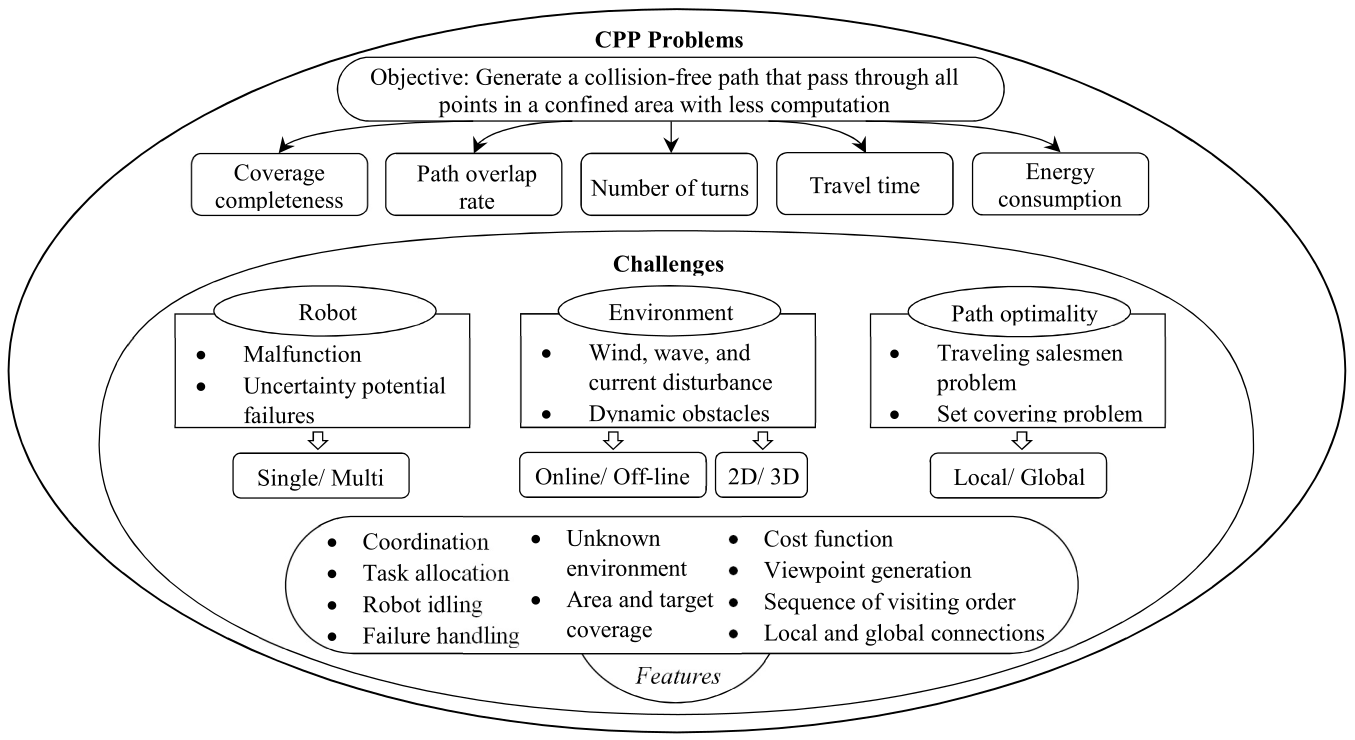
\includegraphics[width=\textwidth]{Images/general/overview_of_CPP.png}
    \caption{The objective and challenges in coverage path planning (CPP) problems.}
    \label{fig:overview_of_CPP}
\end{figure}

Over the years, researchers have developed a myriad of algorithms to address different aspects of path planning, ranging from basic algorithms to more advanced methodologies. CPP algorithms can be categorized into two approaches, classical algorithms, and heuristic-based algorithms. The summarized details of CPP algorithms according to the characteristics of the algorithms as stated in the paper \hyperlink{cite.main_review}{[2]} are classified as shown in (\autoref{fig:classifications_of_CPP}). 

\begin{figure}[htbp]
    \centering
    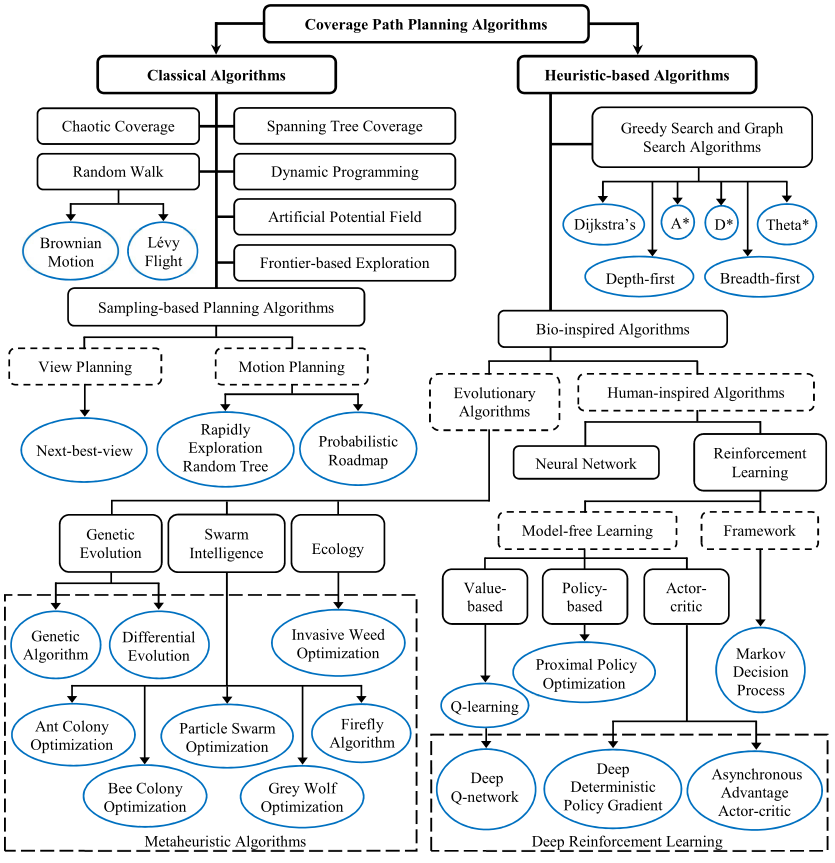
\includegraphics[height=22cm, width=\textwidth]{Images/general/general_classification.png}
    \caption{The classification of coverage path planning (CPP) algorithms.}
    \label{fig:classifications_of_CPP}
\end{figure}

\vspace{3mm}

Several algorithms relevant to coverage path planning for points or regions, which adhere to non-holonomic constraints with the objective of minimizing total route length, computational time, and energy consumption, are discussed below.


\subsection{Dubin's Path}

In the realm of geometric analysis and constrained path planning, the pioneering work of L.E. Dubins stands as a cornerstone, providing profound insights into the properties and characteristics of paths subject to curvature constraints. Dubins' seminal exploration, outlined in the paper \hyperlink{cite.dubins}{[1]}, lays a robust foundation for understanding the fundamental principles governing constrained path planning and provides critical insights into the properties of paths constrained by curvature.

\vspace{3mm}

At the core of Dubins' research lies the concept of R-geodesics, representing paths of minimal length under specified curvature constraints. This notion encapsulates the geometric essence of constrained paths, defining them as combinations of straight lines and circular arcs with a minimum radius of curvature, denoted as R. Dubins' theorem regarding the structure of R-geodesics in two dimensions provides a clear geometric understanding, asserting that such paths consist of no more than three segments, each comprising either a straight line or an arc of a circle with radius R. This theorem delineates the structure of minimal paths and imposes precise constraints on their composition, revealing the inherent simplicity of paths subject to curvature constraints.

\vspace{3mm}

Dubins rigorously proved the existence of R-geodesics using mathematical tools like Ascoli's theorem and concepts from E. Schmidt's proof of A. Schur's Lemma. These proofs confirm the theoretical existence of such paths and illuminate their analytical and geometric properties.

\vspace{3mm}

Dubins' work represents a significant milestone in the study of geometric analysis and constrained path planning, providing not only a solution to a specific geometric problem but also a methodological framework applicable to a broader class of problems in path planning and optimization. Therefore, many extensions of Dubins have been studied since then, integrating with other approaches to solve complex path planning problems. Due to its effectiveness towards curvature constraints and path length minimization, the Dubins path serves as a potential technique to inspire and inform further research into path planning algorithms for agricultural robots.


\subsection{Reeds-Shepp Paths}

Reeds-Shepp paths, introduced by J.A. Reeds and L.A. Shepp in the paper \hyperlink{cite.reeds}{[3]}, offers a flexible solution to optimal path planning for vehicles capable of moving forwards and backwards. Unlike Dubins paths, which only accommodate forward movement, Reeds-Shepp paths enhance maneuverability by incorporating reverse movements, doubling the range of possible maneuvers. This flexibility enables efficient navigation in complex environments, making them ideal for applications like robotics and autonomous vehicle navigation.

\vspace{3mm}

In agricultural robotics, Reeds-Shepp paths are particularly beneficial for tasks like weed removal, where precise navigation is essential. Their flexibility allows for efficient navigation through narrow spaces and around obstacles, reducing time and energy consumption. Reeds and Shepp's comprehensive analysis of Reeds-Shepp paths laid the foundation for subsequent research in optimal control and path planning, emphasizing the importance of considering a vehicle's full range of capabilities.





\subsection{Travelling Salesman Problem (TSP) with Neighborhoods} 

The Traveling Salesman Problem (TSP) represents a classic conundrum in optimization, challenging researchers to find the most efficient route for a salesman to visit a set of locations and return to the starting point while minimizing the total distance traveled. Renowned for its computational complexity and practical applications in logistics and route planning, the TSP has spurred numerous investigations into variants that more accurately reflect real-world scenarios.

\vspace{3mm}

One such variant, explored in the paper \hyperlink{cite.TSPN}{[4]}, introduces the concept of TSP with neighborhoods (TSPN). In this formulation, destinations are not singular points but rather areas or neighborhoods, complicating the problem by requiring the salesman to visit each neighborhood at least once without specifying exact points for each visit. TSPN is particularly relevant as it mirrors the challenge of navigating through regions (fields with weeds) rather than fixed points.

\vspace{3mm}

To address the challenges posed by TSPN, the paper introduces innovative approximation algorithms tailored to different types of neighborhoods, such as line segments or complex shapes described as "fat" regions. A notable contribution is the development of a constant factor approximation algorithm for neighborhoods represented as line segments, signifying a significant advancement in the field of geometric optimization.

\vspace{3mm}

A significant contribution of the paper is the m-guillotine method, which recursively subdivides the plane to approach a near-optimal solution. This method, along with key theoretical insights, underpins the algorithms' effectiveness in solving TSPN. However, it is essential to note that the TSPN problem is NP-hard, and the proposed algorithms provide only approximation solutions. While TSPN works with regions instead of points and strives to find the optimal solution, it does not explicitly consider the curvature constraints inherent in robotic path planning scenarios.











\subsection{Traveling Salesperson Problems for Dubins’ vehicle.}



After TSPN evolved from TSP, the challenges associated with optimal path planning for Dubins' vehicles, constrained by their minimum turning radius, have garnered significant attention. The paper \hyperlink{cite.TSP_with_dubins}{[5]} offers a thorough examination of these challenges and introduces innovative methodologies to overcome them.

\vspace{3mm}


At the core of this paper are two fundamental problems: the point-to-point shortest path problem (PTP) and the traveling salesperson problem (TSP) tailored for Dubins’ vehicles. These problems are crucial for developing algorithms capable of computing optimal or near-optimal paths for vehicles subject to nonholonomic constraints. the paper tackles the traveling salesperson problem (TSP) for Dubins’ vehicles, wherein the vehicle must visit a predefined set of locations in the most efficient route without revisiting any point. Acknowledging the computational complexity of exact solutions for larger point sets, the authors explore heuristic and approximation algorithms to efficiently approximate solutions.

\vspace{3mm}

The methodology outlined in the paper integrates rigorous mathematical frameworks and computational geometry to address the complexities of path planning for Dubins’ vehicles. By synthesizing Dubins constraints with the Traveling Salesperson Problem (TSP), the study offers a cohesive approach that bridges theoretical insights with practical solutions. this paper constitutes a significant contribution to the literature on path planning for nonholonomically constrained vehicles, paving the way for further advancements in navigating Dubins’ vehicles efficiently and effectively.











\subsection{Dubins Traveling Salesman Problem with Neighborhoods}

To address the challenges posed by regions in the Dubins Traveling Salesman Problem (DTSP), the paper \hyperlink{cite.DTSPN}{[6]} introduces a tailored formulation termed the Dubins Touring Regions Problem (DTRP). This novel approach aims to determine an optimal sequence of configurations for entering and exiting regions, all while minimizing the total path length. Unlike the conventional Traveling Salesman Problem (TSP), which focuses on finding the shortest route visiting a set of points, the DTSPN involves regions or neighborhoods, necessitating the vehicle to access each region at least once. This problem holds significant relevance in various applications, including autonomous drone surveillance, delivery systems, and robotic exploration, where vehicles must efficiently traverse specified areas while adhering to nonholonomic constraints.

\vspace{3mm}

The proposed algorithm for solving the DTRP leverages local iterative optimization techniques, taking into account the unique dynamics of Dubins vehicles. It begins with an initial sequence of region visits derived from solving an Euclidean TSP (ETSP), which serves as a proxy for the region centers. The algorithm then iteratively refines the entry and exit configurations to minimize the total tour length.

\vspace{3mm}

A key aspect of the solution method is its decoupled approach, optimizing the heading and position of each entry point independently. This simplification, facilitated by mathematical techniques that project the problem into a more manageable form, allows for efficient local optimization. The algorithm iterates until no further improvements can be made or a termination criterion is met, incorporating strategies to escape local minima by adjusting vehicle headings and repositioning at region boundaries.

\vspace{3mm}

Empirical validation of the algorithm demonstrates its effectiveness and efficiency across various scenarios, including different region shapes and configurations, particularly in dense environments where regions are close together. Comparative analysis against existing evolutionary algorithms showcases the proposed method's ability to produce high-quality solutions with significantly reduced computational time, making it suitable for real-time applications on modest hardware, such as onboard computers in UAVs.

\vspace{3mm}

Despite its capability to generate near-optimal paths while adhering to the non-holonomic constraints, the algorithm exhibits notable drawbacks in terms of computational efficiency. For instance, computing a near-optimal path for 30 regions may require over a minute, and the algorithm's performance further deteriorates with an increasing number of points, especially when they are closely positioned. Moreover, the algorithm's limitation in considering the overlap of regions represents a critical drawback, as it fails to account for this aspect in real-world scenarios, thereby impacting the path planning accuracy and efficiency.




\subsection{DTSPN with Overlappped Regions}



The paper \hyperlink{cite.overlap}{[7]} introduces the Intersecting Regions Algorithm (IRA) to address the challenges posed by intersecting regions in DTSPN. By explicitly considering the overlap among regions, IRA offers a more comprehensive solution compared to traditional methods. It leverages sampling within intersecting regions to construct feasible tours for autonomous vehicles, resulting in optimized route selection and more efficient path planning.

\vspace{3mm}

Furthermore, IRA reduces the computational complexity associated with path planning by adopting a polynomially scalable algorithmic structure. This scalability ensures IRA's viability even in scenarios with numerous regions of interest, where computational resources are limited. Monte Carlo simulations validate IRA's practical utility, showcasing significant performance enhancements, particularly in scenarios with high degrees of region overlap. However, despite its advancements, IRA still encounters challenges when dealing with a large number of points and close proximity points. These limitations highlight avenues for further research and development to enhance the algorithm's robustness and efficiency in addressing complex DTSPN scenarios.








\subsection{Path planning in confined spaces}


Navigating narrow and complex environments presents challenges for non-holonomic vehicles. In the paper \hyperlink{cite.mapping}{[8]}, the authors propose a path planning method tailored to address these challenges, focusing on generating paths with continuous curvature to ensure smooth operation in confined spaces.

\vspace{3mm}

The proposed method adopts a two-phase planning approach combining global and local strategies for efficient navigation. In the first phase, the authors employ the RTR (Rotate-Translate-Rotate) planner, a variation of the Rapidly Exploring Random Tree (RRT) method. This planner generates paths consisting of straight movements and in-place turning, simplifying complex maneuvering for navigating constrained spaces.

\vspace{3mm}

In the second phase, the global path is refined using the TTS local planning procedure. This planner approximates the initial path with a sequence of paths adhering to the vehicle's curvature constraints, ensuring smooth and feasible trajectories. The TTS planner can generate paths with continuous curvature turns (CC-turns) and straight segments, offering flexibility adaptable to various environmental constraints.

\vspace{3mm}

The paper also emphasizes maintaining similarity between global and local trajectories to avoid sudden changes in the path and ensure smooth passage through narrow regions. Ultimately, the objective is to enhance the capabilities of autonomous vehicles to operate safely and efficiently in diverse scenarios, thereby improving their practicality for everyday use.

